\chapter{Dark matter interpretation}
\label{chap:results}

This chapter covers the results and interpretation of the fitting procedure described in the previous chapter, including the upper limits on signal cross sections for the \ttDM process in the dilepton channel presented in \SectionRef{sec:UL}. The results presented in this work have been combined with the \ttDM searches performed using the all-hadronic and lepton+jets \ttbar decay modes as presented in~\cite{CMS-PAS-EXO-16-049}. The sensitivity in the combined search is driven by the all-hadronic channel, however this work contributes significantly to the sensitivity for scalar mediated signal models with $\mMed<50\:\GeV$, where the softer signal \MET spectra are exploited. The CMS \ttDM search performed in 2016 provides the best sensitivity for low mediator mass models when compared with other spin-0 $\text{Mono}$-$X$ LHC searches, including monojet~\cite{Sirunyan:2017jix}. \SectionRef{sec:comparetoDD} presents the results in the same planes as results from dedicated direct DM detection experiments. 

\section{Upper limits on \ttllDM production at the LHC}
\label{sec:UL}

The background-only post-fit yields presented in \TableRef{tab:cat-hi_postfit_yields} and \TableRef{tab:cat-lo_postfit_yields} reveal an observed yield compatible with the events expected from SM backgrounds, within statistical and systematic uncertainties. Thus, without a significant excess of events expected over the SM processes, $95\%$ $\textrm{CL}_{s}$ upper limits on the signal strength parameter $\mu$, defined in \SectionRef{subsec:signal} as the ratio of the observed cross section to the theoretical model cross section, are set. The expected and observed upper limits on $\mu$ for signal models with varying S and PS mediator masses and $\mDM=1\:\GeV$ are listed in \TableRef{tab:results}, along with the $\pm\:1\sigma$ and $\pm\:2\sigma$ uncertainties on the expected limit. Recalling the discussion in \SectionRef{sec:simpmodels}, the more stringent limit at low mediator mass for S compared to PS models can be understood as a manifestation of the order of magnitude difference in cross section between the S and PS mediated DM production at low mass. A similar reasoning is followed at high mediator mass, when the cross section for PS models becomes equivalent or marginally larger than the S mediated production rate, where it is observed that the upper limit is more comparable between S and PS models than at low mass. The results shown in the tables are visualized in~\FigureRef{fig:scalar_results} and~\FigureRef{fig:pseudo_results} as a function of \mMed, where the couplings are assumed to be $\gq = \gDM = 1$ and $\mDM=1\:\GeV$. The logarithmic scaling of the x and y axes in \FigureRef{fig:scalar_results} and \FigureRef{fig:pseudo_results} somewhat conceal the sharp rise in the expected and observed upper limits beginning at $\mMed\approx 300\:\GeV$. However, following the discussion in \SectionRef{sec:BSM} regarding the enhancement of \ttbar production to the minimal mediator width in the region $\mMed > 2\mtop$, this rising trend is unsurprising, as the \XX production mode is no longer dominant and therefore the cross section for DM production drops off drastically. The rise in upper limit is also noticeably sharper for the S compared to the PS mediated signal models owing to the kinematic suppression of S compared to PS production as discussed in \SectionRef{sec:simpmodels}. In the high \mttll category post-fit \MET distributions shown in~\FigureRef{fig:postfit_hi}, a modest excess of observed events over the expected SM backgrounds can be seen at high \MET for both flavor categories. As a result, this causes the observed upper limits for both S and PS mediators to be consistently $15-25\%$ weaker than the corresponding expected limits across the \mMed range in the absence of a signal. Contrary to mass peak searches where the postulated signal may be localized in a window of the mass distribution being fit, this search would anticipate an excess over a non-localized range of the \MET distribution, thus also explaining the uniformity of the weaker observed compared to expected limits. The range of \mMed are referred to as excluded by the search, when the upper limit on $\mu$ is less than 1. As can be seen in~\FigureRef{fig:scalar_results} and~\FigureRef{fig:pseudo_results}, the observed (expected) $95\%$ $\textrm{CL}_{s}$ exclusions for a S mediator are $\mMed<74(99)\:\GeV$, while for a PS mediator, the expected exclusion is $m_{a}<50\:\GeV$, and no exclusion is observed. 

\begin{table}
  \begin{tabular}{|l|c|c|c|c|}
    \hline
    Model (\mMed,\mDM) [GeV] &   Obs.  &    Exp. &  $[  -1\sigma, +1\sigma  ]$ &  $[  -2\sigma, +2\sigma  ]$ \\ \hline
    S  10,   1 &      0.72 &     0.59 &   $[   0.41,    0.89]$ &  $[   0.30,    1.32]$ \\
    S  20,   1 &      0.64 &     0.51 &   $[   0.35,    0.76]$ &  $[   0.25,    1.11]$ \\
    S  50,   1 &      0.74 &     0.62 &   $[   0.43,    0.94]$ &  $[   0.31,    1.36]$ \\
    S 100,   1 &      1.29 &     1.01 &   $[   0.69,    1.51]$ &  $[   0.51,    2.19]$ \\
    S 200,   1 &      2.97 &     2.40 &   $[   1.64,    3.58]$ &  $[   1.19,    5.22]$ \\
    S 300,   1 &      5.64 &     4.61 &   $[   3.16,    6.91]$ &  $[   2.30,   10.11]$ \\
    S 500,   1 &     22.93 &    18.74 &   $[  12.78,   28.52]$ &  $[   9.26,   42.20]$ \\ 
    \hline
    PS  10,   1 &      1.16 &     0.92 &   $[   0.63,    1.38]$ &  $[   0.46,    2.01]$ \\
    PS  20,   1 &      1.16 &     0.92 &   $[   0.63,    1.38]$ &  $[   0.46,    2.01]$ \\
    PS  50,   1 &      1.26 &     1.00 &   $[   0.69,    1.50]$ &  $[   0.50,    2.19]$ \\
    PS 100,   1 &      1.49 &     1.18 &   $[   0.81,    1.77]$ &  $[   0.59,    2.59]$ \\
    PS 200,   1 &      2.45 &     1.95 &   $[   1.33,    2.93]$ &  $[   0.96,    4.30]$ \\
    PS 300,   1 &      3.99 &     3.23 &   $[   2.19,    4.89]$ &  $[   1.60,    7.22]$ \\
    PS 500,   1 &     22.29 &    18.06 &   $[  12.15,   27.49]$ &  $[   8.78,   41.31]$ \\\hline
  \end{tabular}
  \caption{Observed and expected upper limits at $95\%$ $\textrm{CL}_{s}$ on $\mu$ as a function of scalar (S) and pseudoscalar (PS) mediator masses for $\mDM=1\:\GeV$ with $\pm\:1\sigma$ and $\pm\:2\sigma$ uncertainties on the expected limits.}
  \label{tab:results}
\end{table}

\begin{figure}
  \centering
  \subfloat[][Upper limits for scalar mediators]{
    \label{fig:scalar_results}
    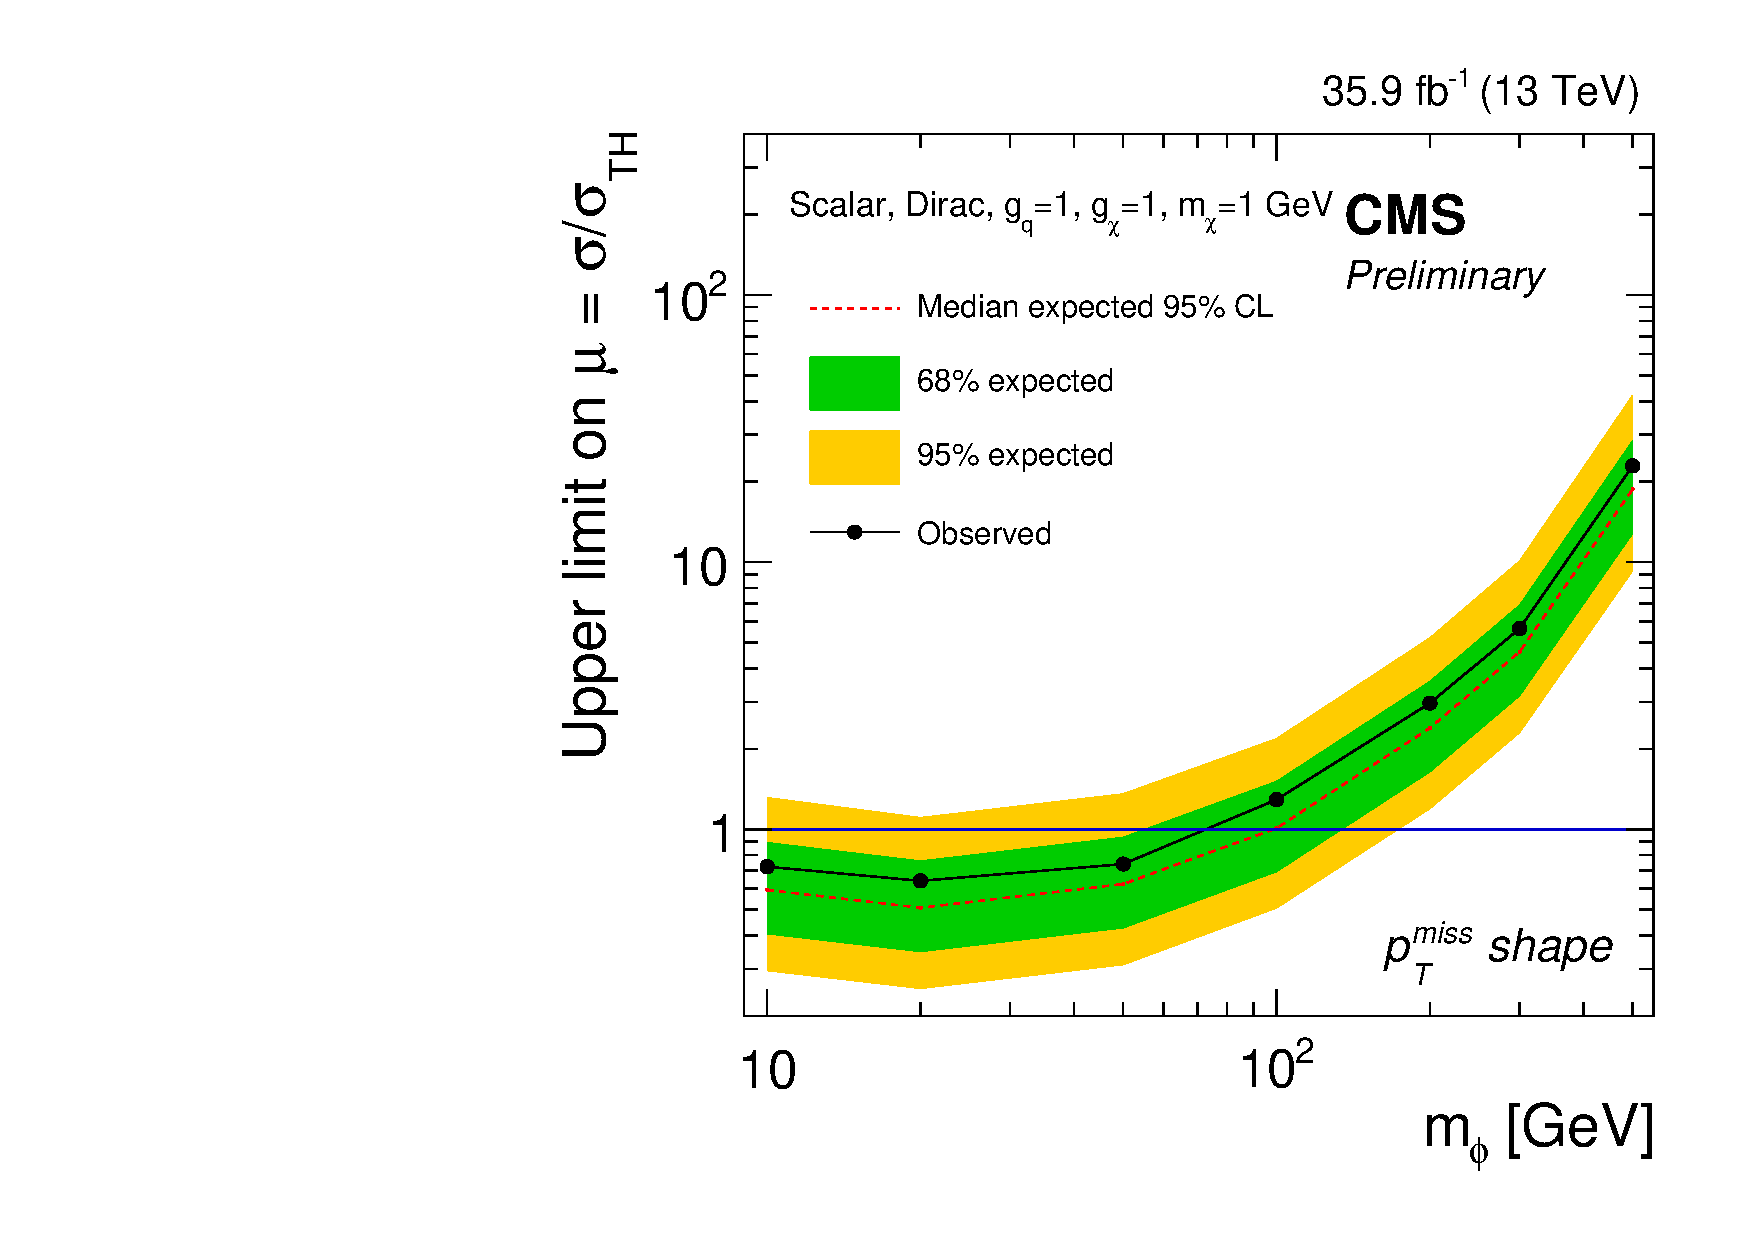
\includegraphics[width=0.6\textwidth]{figs/dilepton_S_NLO_limits.pdf}
  } 
  \hspace{1 cm}
  \subfloat[][Upper limits for pseudoscalar mediators]{
    \label{fig:pseudo_results}
    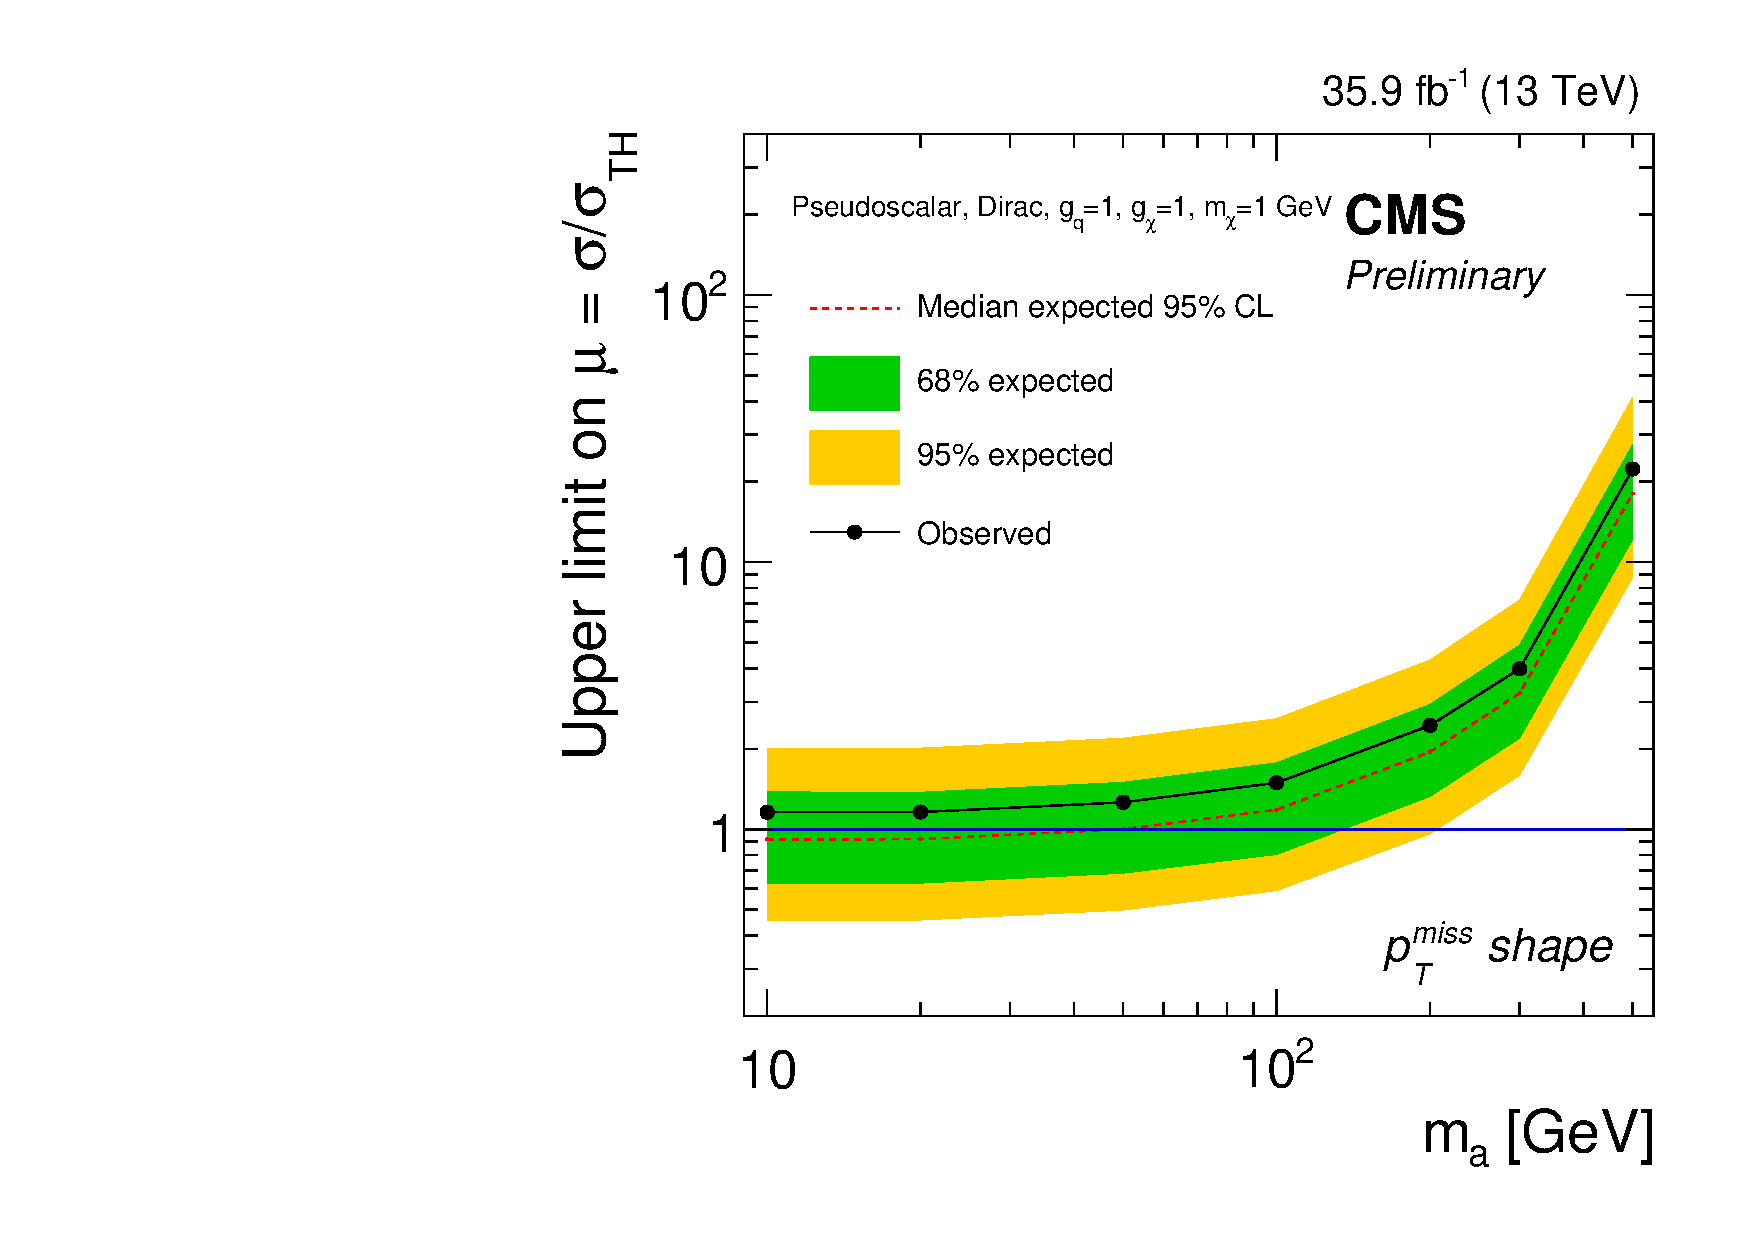
\includegraphics[width=0.6\textwidth]{figs/dilepton_PS_NLO_limits.pdf}
  }
  \caption{The expected (red dashed) and observed (solid black) $95\%$ $\textrm{CL}_{s}$ upper limits on the \ttDM signal strength in the dilepton channel for various~\protect\subref{fig:scalar_results} scalar and~\protect\subref{fig:pseudo_results} pseudoscalar mediator masses where $\mDM=1\:\GeV$ and $\gq = \gDM = 1$ is assumed. The green (yellow) band represents the $68\%$ ($95\%$) interval of probability around the expected limit. The results are obtained using $35.9\:\textrm{fb}^{-1}$ collected by the CMS detector in 2016.}
\end{figure}

\clearpage

The 1D mediator exclusion range observed and expected for the scalar mediated \ttDM signal in \FigureRef{fig:scalar_results} is expanded into a 2D contour as a function of \mMed and \mDM as shown in~\FigureRef{fig:2Dexclusion}. The 1D upper limit curves can be thought of as slices across the x axis (\mMed) for a given y value (\mDM) in the 2D plane. The solid (finely dashed) contour encloses the region where the observed (expected) upper limit on $\mu$ is less than 1. The triangular nature of the exclusion contour is based on the grounding assumption that the kinematics for a given \mMed do not change dramatically as a function of \mDM, provided the DM particles are produced sufficiently on-shell. In addition, as the on/off-shell threshold (dashed diagonal) line is approached, both the width as given by~\EquationRef{eq:width} and the cross section fall monotonically and plateau at very small, but non-zero values, thus the exclusion contour runs close to the diagonal but does not cross. The narrow mediator width would nominally enhance the cross section in such a limiting case as the threshold regime, however the allowable phase space for the decay products is greatly reduced at $\mMed \approx 2\mDM$, ultimately suppressing the total cross section.

\begin{figure}
  \centering
  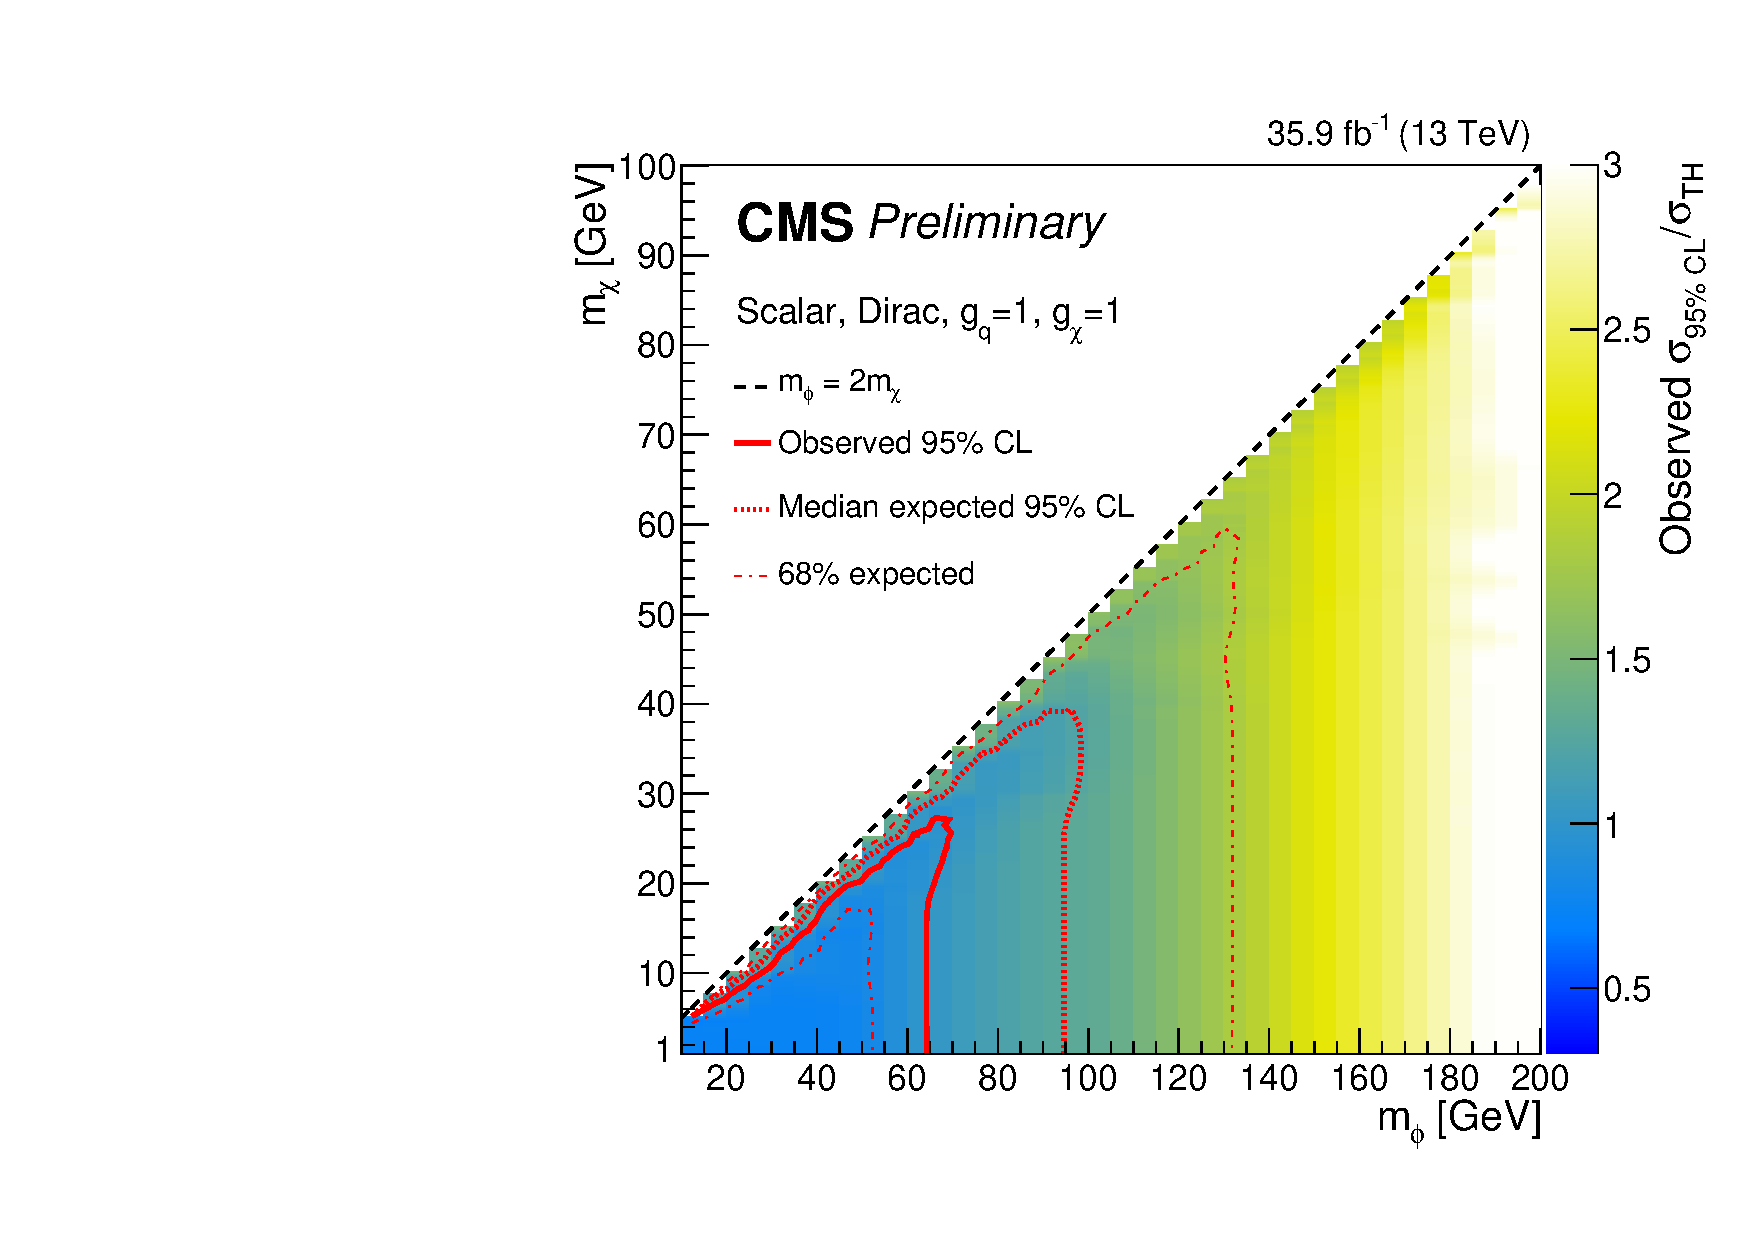
\includegraphics[width=0.65\textwidth]{figs/dilept_inc_S_limits2D_NLO.pdf}
  \caption{The exclusion limits at $95\%$ $\textrm{CL}_{s}$ on the signal strength parameter $\mu$ for the \ttDM process in the dilepton channel, computed as a function of the mediator mass and DM mass, assuming a scalar mediator. The mediator couplings are assumed to be $\gq=\gDM=1$.}
  \label{fig:2Dexclusion}
\end{figure}

\clearpage 

\section{Comparison with direct detection}
\label{sec:comparetoDD}

The problem of DM is one of many dimensions, thus many independent and complementary approaches are required in attempts to solve it. Although this work does not provide evidence for a potential WIMP discovery, the role that collider detection plays in the search for DM is important in relation to ID and DD methods. The latter are necessary for determining the existence of DM particles whether through nuclear scattering, or annihilation to ordinary particles. From one perspective, these approaches can establish DM particle existence and provide information on the SM particles it may interact with. Particle accelerator production of DM then allows for the detailed study of DM particle properties under a controled environment. Characterization of DM particle properties would subsequently allow particle physicists to make an appropriate decision on the theoretical framework that contains the new particle. Conversely, supposing a WIMP discovery is made via a collider search, such as a weakly interacting neutralino, and its properties such as decay modes, spin-parity, and mass can be characterized at the LHC; it then remains for the ID and DD experiments to ascertain that the new particle is indeed a DM particle. As a result of the complementarity of the approaches, the interpretation of results from different detection methods is instrumental in mapping out the search phase space.

To facilitate the comparison with constraints from DD experiments of the type mentioned in \SectionRef{subsec:DD}, the exclusion contours obtained from the scalar \ttDM model as shown in~\FigureRef{fig:2Dexclusion} are calculated at $90\%$ $\textrm{CL}_{s}$. Subsequently, the upper limits on $\mu$ are translated to upper limits on the SI DM-nucleon scattering cross section via the approach taken from~\cite{Boveia:2016mrp} as briefly described in the proceeding section.

\subsection{Spin-indepedent comparison}
\label{subsec:SIcase}

The general form of the SI DM-nucleon scattering cross section is,

\begin{equation}
  \sigma_{\textrm{SI}} = \frac{f^{2}(\gq)\gDM^{2}m_r^2}{\pi\mMed^{4}}
  \label{eq:DDtranslation}
\end{equation}

where $m_r = m_{N}\mDM/(m_{N}+\mDM)$ is the DM-nucleon reduced mass, as in \EquationRef{eq:diffxsec}, with $m_{N} \simeq 0.939\:\GeV$ being the approximate nucleon mass. The mediator-nucleon coupling, denoted by $f(\gq)$, has a non-trivial dependence on the mediator-quark couplings and the Higgs boson vacuum expectation value, so the full definition is ommitted. However, using the most state-of-the-art values for these dependencies from~\cite{Hoferichter:2015dsa} and~\cite{Junnarkar:2013ac}, the numerical value of $f(\gq)$ is,

\begin{equation}
  f(\gq) = 1.16 \times 10^{-3} \gq.
\end{equation} 

Thus,\EquationRef{eq:DDtranslation} takes the form,

\begin{equation}
  \sigma_{\textrm{SI}} \simeq 6.9 \times 10^{-43} \Big(\frac{\gq\gDM}{1}\Big)^{2}\Big(\frac{125\:\GeV}{\mMed}\Big)^{4}\Big(\frac{m_{r}}{1\:\GeV}\Big)^{2}.
  \label{eq:xsecDDtrans}
\end{equation}

As a result, the upper limit on $\mu$ for the scalar-mediated \ttllDM process is presented as an exclusion bound in the \mDM-$\sigma_{\textrm{SI}}$ plane in~\FigureRef{fig:DDplot}. The assumptions made in the translation include that the DM particle is a Dirac fermion, the coupling values are $\gq = \gDM = 1$, and the CMS expected and observed exclusions are calculated at $90\%$ $\textrm{CL}_{s}$, as is standard in the DD community. In the translation performed using \EquationRef{eq:xsecDDtrans}, for a given \mDM, the \mMed value used is the one for which the upper limit on $\mu$ is equal to one. At $\mDM \gtrsim 5\:\GeV$, the larger dual-phase noble gas detectors discussed in~\SectionRef{subsec:DD} greatly constrain the search phase space. In contrast, the collider limits presented in this work are the most constraining at low DM mass, a fact well-supported by the strong constraints at low \mMed as seen in the upper limit curve in~\FigureRef{fig:scalar_results} where $\mDM=1\:\GeV$. 

\begin{figure}
  \centering
  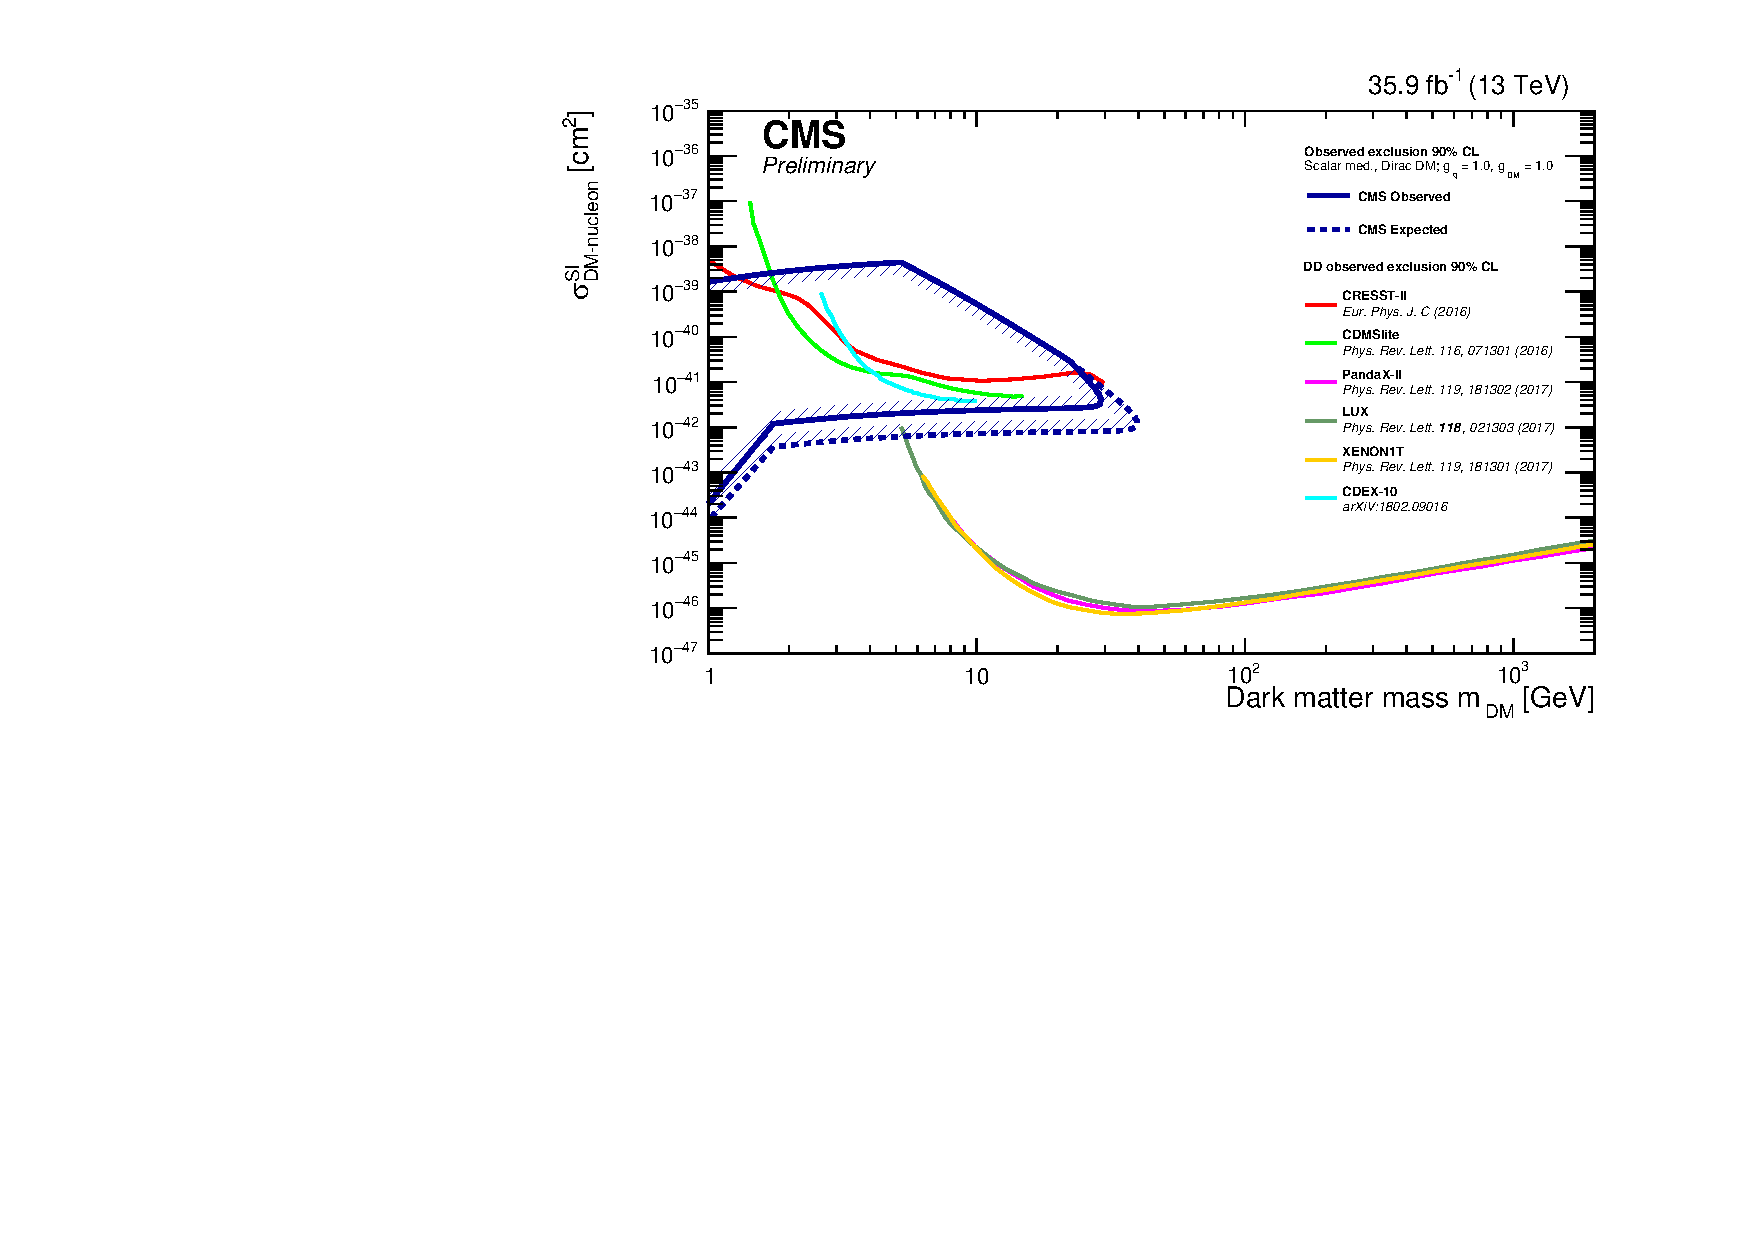
\includegraphics[width=\textwidth]{figs/SIS_CMSDD_Summary.pdf}
  \caption{A comparison of the \ttllDM scalar-mediated results (CMS expected and observed lines) to the exclusion contours of the LUX, PandaX-II, XENON1T, CDEX-10, CDMSLite, and CRESST-II limits in the \mDM-$\sigma_{\textrm{SI}}$ plane. The DM particle is assumed to be a Dirac fermion and $\gq = \gDM =1$.}
  \label{fig:DDplot}
\end{figure}
